\chapter{Esercizio 8}
\section{Prova di esame del 19 dicembre 2024}
\subsection{Traccia}
 Un sistema è composto da 2 nodi, A e B. A include una ROM (progettata come macchina sequenziale con READ sincrono) di 8 locazioni da 4 bit, mentre B include un sommatore 
parallelo in grado di effettuare la somma di 2 stringhe di 4 bit ciascuna e un registro R di 4 bit. Il sistema opera come segue: all’arrivo di un segnale di start,  A inizia a prelevare gli elementi ROM[i] dalla propria memoria e li invia, uno alla volta, a B mediante handshaking. B somma progressivamente le stringhe ricevute utilizzando il sommatore e alla fine inserisce il risultato nel registro R.
\subsection{Progettazione}
Il progetto di questo sistema si compone di due nodi fondamentali: il nodo A e il nodo B che comunicano tramite handshaking.\\
Il nodo A si compone di una memoria di sola lettura (ROM), un contatore e un'unità di controllo che gestisce l'interazione;\\
il nodo B si compone di un sommatore \textit{Carry Look Ahead}, di un registro e di una unittà di controllo per le rispettive operazioni.\\
Di seguito viene mostrata lo schema a blocchi del sistema, con la suddivisione in due nodi distinti.
\begin{figure}[H]
	\centering
	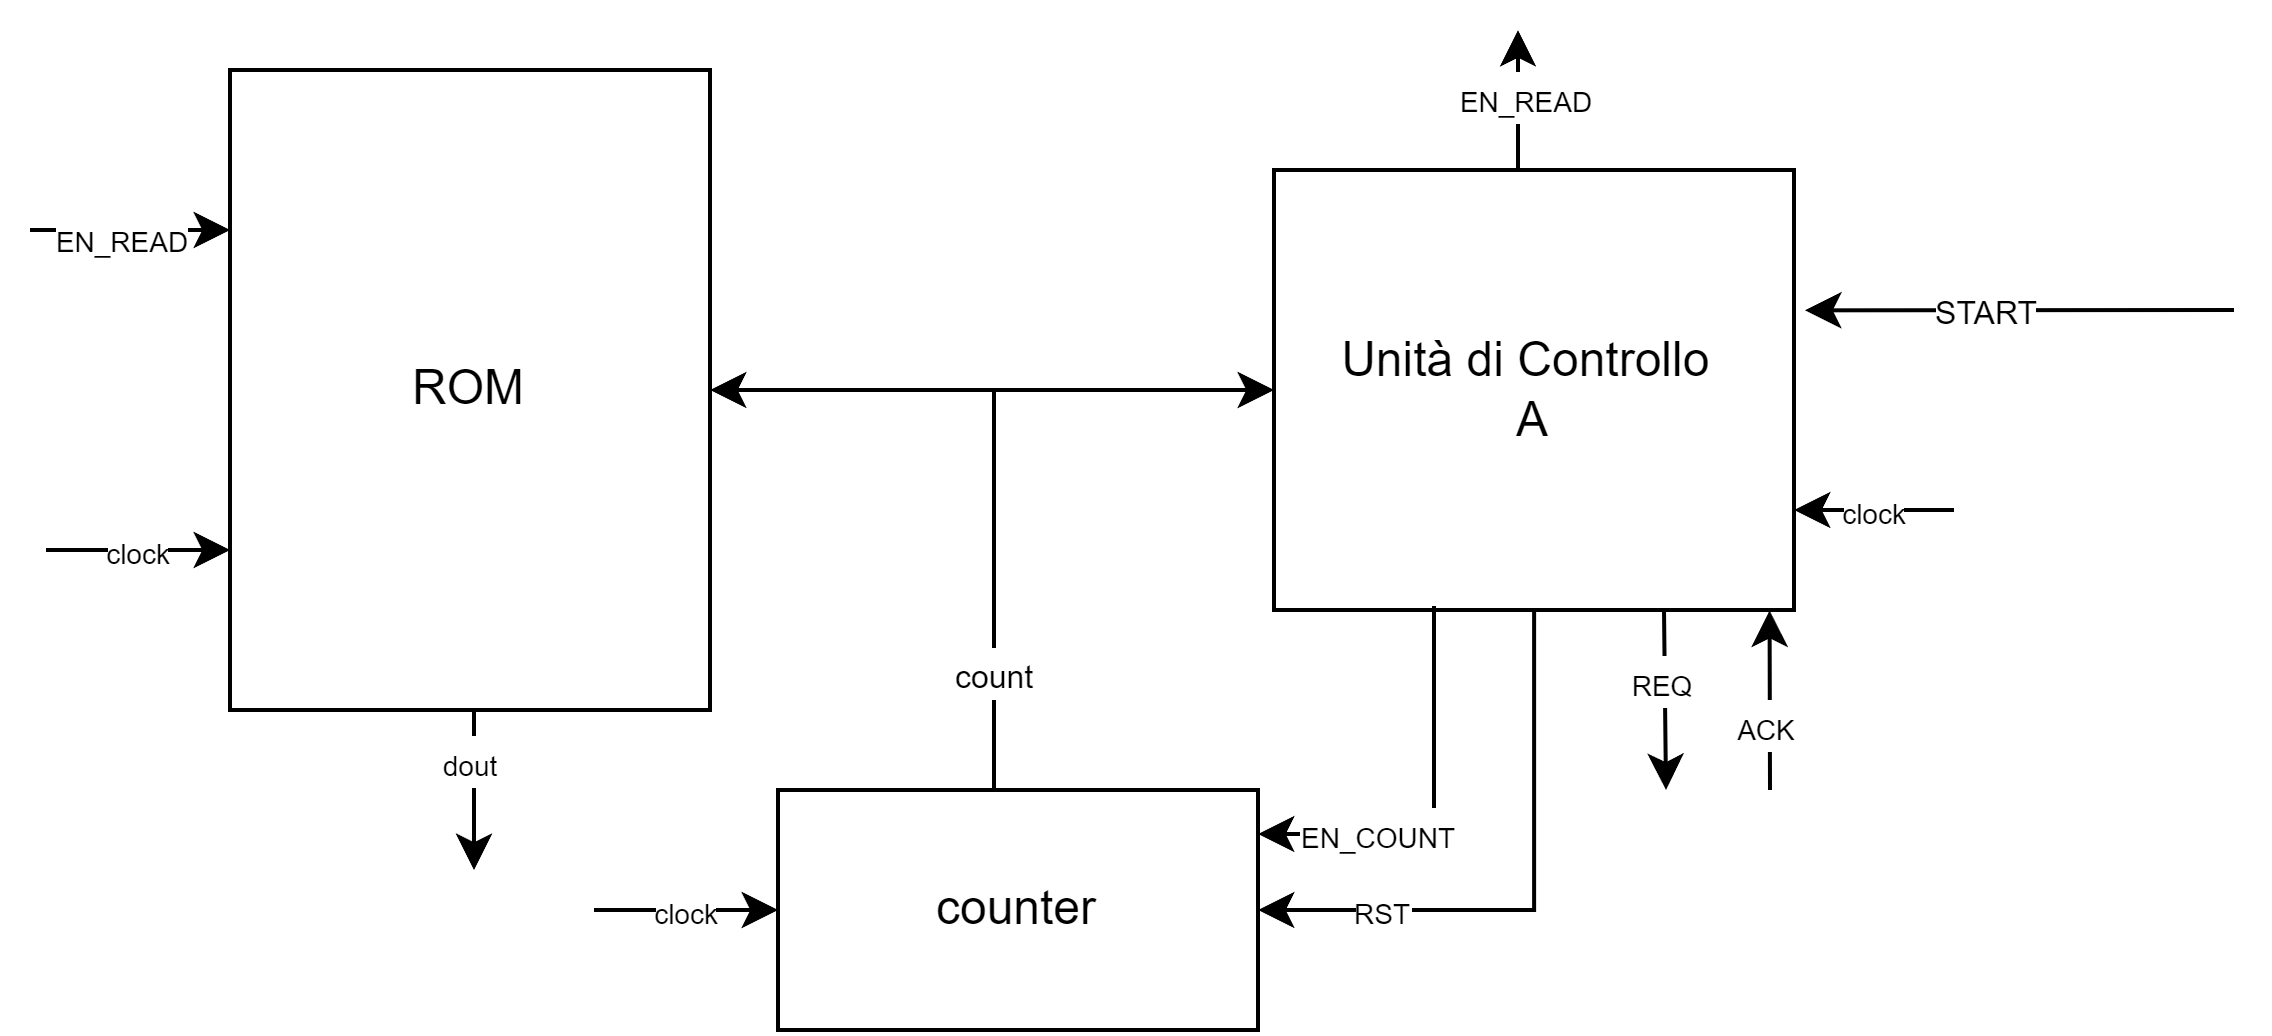
\includegraphics[width=1\textwidth]{img/preappDicembre/Preapp_NodoA}
	\caption{Schema a blocchi: nodo A}
	\label{wf_preapp} 
\end{figure}
\begin{figure}[H]
	\centering
	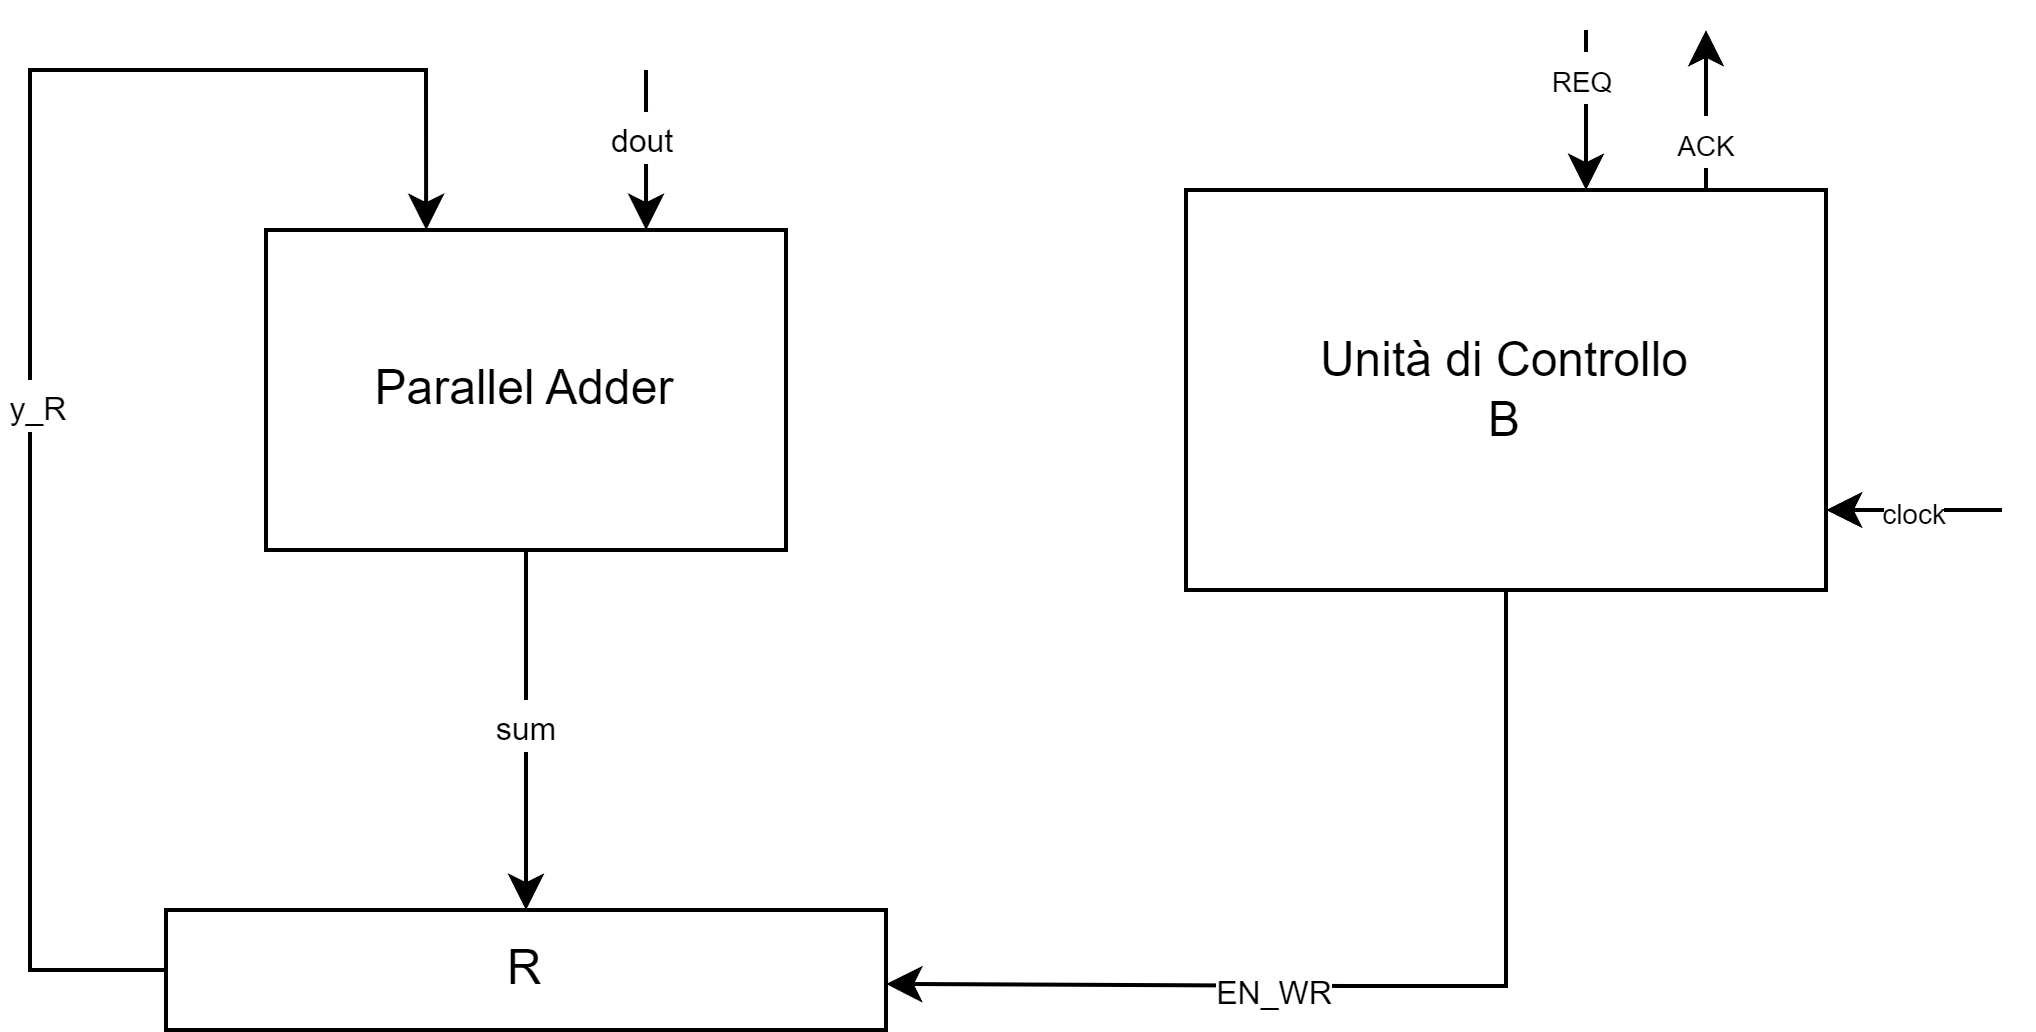
\includegraphics[width=1\textwidth]{img/preappDicembre/Preapp_NodoB}
	\caption{Schema a blocchi: nodo B}
	\label{wf_preapp} 
\end{figure}
Nella fase di progettazione, si creano anche gli automi relativi alle unità di controllo dei due nodi, qui mostrati:
\begin{figure}[H]
	\centering
	\includegraphics[width=1\textwidth]{img/preappDicembre/Preapp_automaA}
	\caption{Automa unità di controllo: nodo A}
	\label{wf_preapp} 
\end{figure}
\begin{figure}[H]
	\centering
	\includegraphics[width=1\textwidth]{img/preappDicembre/Preapp_automaB}
	\caption{Automa unità di controllo: nodo B}
	\label{wf_preapp} 
\end{figure}
\subsection{Implementazione}
Per l'implementazione si parte dal nodo A: \\
partendo dall'unità operativa, essa è composta da una ROM e da un contatore. Si mostrano i rispettivi codici.
\begin{code}
    \inputminted[frame=lines, framesep=2mm, baselinestretch=1.2, bgcolor=LightGray, fontsize=\footnotesize, linenos]{vhdl}{vhdl_files/preappDicembre/ROM.vhd}
    \caption{ROM.vhdl}
    \label{lst:mux_2_1}
\end{code}

\begin{code}
    \inputminted[frame=lines, framesep=2mm, baselinestretch=1.2, bgcolor=LightGray, fontsize=\footnotesize, linenos]{vhdl}{vhdl_files/preappDicembre/count_8.vhd}
    \caption{Contatore modulo 8.vhdl}
    \label{lst:mux_2_1}
\end{code}
Tali componenti vengono collegati tra loro nell'\textit{unità operativa}:
\begin{code}
    \inputminted[frame=lines, framesep=2mm, baselinestretch=1.2, bgcolor=LightGray, fontsize=\footnotesize, linenos]{vhdl}{vhdl_files/preappDicembre/unita_operativa.vhd}
    \caption{CUnità operativa di A in vhdl}
    \label{lst:mux_2_1}
\end{code}
Per la gestione delle abilitazioni, si utilizza un'unità di controllo, come si vede dallo schema a blocchi nel paragrafo precedente:
\begin{code}
    \inputminted[frame=lines, framesep=2mm, baselinestretch=1.2, bgcolor=LightGray, fontsize=\footnotesize, linenos]{vhdl}{vhdl_files/preappDicembre/UCA.vhd}
    \caption{Control Unit di A.vhdl}
    \label{lst:mux_2_1}
\end{code}
Il nodo A nel suo complesso sarà implementato in questo modo:
\begin{code}
    \inputminted[frame=lines, framesep=2mm, baselinestretch=1.2, bgcolor=LightGray, fontsize=\footnotesize, linenos]{vhdl}{vhdl_files/preappDicembre/A.vhd}
    \caption{nodo A.vhdl}
    \label{lst:mux_2_1}
\end{code}
Si procede ora con l'implementazione del nodo B, le cui componenti sono un registro R per lo storage del risultato e un Carry Look Ahead:
\begin{code}
    \inputminted[frame=lines, framesep=2mm, baselinestretch=1.2, bgcolor=LightGray, fontsize=\footnotesize, linenos]{vhdl}{vhdl_files/preappDicembre/register.vhd}
    \caption{register.vhdl}
    \label{lst:mux_2_1}
\end{code}
Il sommatore è stato realizzato con un approccio strutturale, a partire da full adder:
\begin{code}
    \inputminted[frame=lines, framesep=2mm, baselinestretch=1.2, bgcolor=LightGray, fontsize=\footnotesize, linenos]{vhdl}{vhdl_files/preappDicembre/full_adder.vhd}
    \caption{full\_adder.vhdl}
    \label{lst:mux_2_1}
\end{code}

\begin{code}
    \inputminted[frame=lines, framesep=2mm, baselinestretch=1.2, bgcolor=LightGray, fontsize=\footnotesize, linenos]{vhdl}{vhdl_files/preappDicembre/CarryLookAhead.vhd}
    \caption{CarryLookAhead.vhdl}
    \label{lst:mux_2_1}
\end{code}
Si mostra ora il codice dell'unità operativa:
\begin{code}
    \inputminted[frame=lines, framesep=2mm, baselinestretch=1.2, bgcolor=LightGray, fontsize=\footnotesize, linenos]{vhdl}{vhdl_files/preappDicembre/unita_operativaB.vhd}
    \caption{unità operativa di B in vhdl}
    \label{lst:mux_2_1}
\end{code}
Come già visto, per la gestione delle abilitazioni e del funzionamento si utilizza un unità di controllo, modellata sulla base degli automi progettati nel paragrafo precedente.
\begin{code}
    \inputminted[frame=lines, framesep=2mm, baselinestretch=1.2, bgcolor=LightGray, fontsize=\footnotesize, linenos]{vhdl}{vhdl_files/preappDicembre/UCB.vhd}
    \caption{Control Unit di A.vhdl}
    \label{lst:mux_2_1}
\end{code}
Il nodo B nel suo complesso viene implementato in questo modo:
\begin{code}
    \inputminted[frame=lines, framesep=2mm, baselinestretch=1.2, bgcolor=LightGray, fontsize=\footnotesize, linenos]{vhdl}{vhdl_files/preappDicembre/B.vhd}
    \caption{nodo B.vhdl}
    \label{lst:mux_2_1}
\end{code}
Il sistema compolessivo composto dai due nodi creato in precedenza si implementa come segue:
\begin{code}
    \inputminted[frame=lines, framesep=2mm, baselinestretch=1.2, bgcolor=LightGray, fontsize=\footnotesize, linenos]{vhdl}{vhdl_files/preappDicembre/AplusB.vhd}
    \caption{AplusB.vhdl}
    \label{lst:mux_2_1}
\end{code}
Si osserva anche lo schematic complessivo generato dall'ambiente Vivado:
\begin{figure}[H]
	\centering
	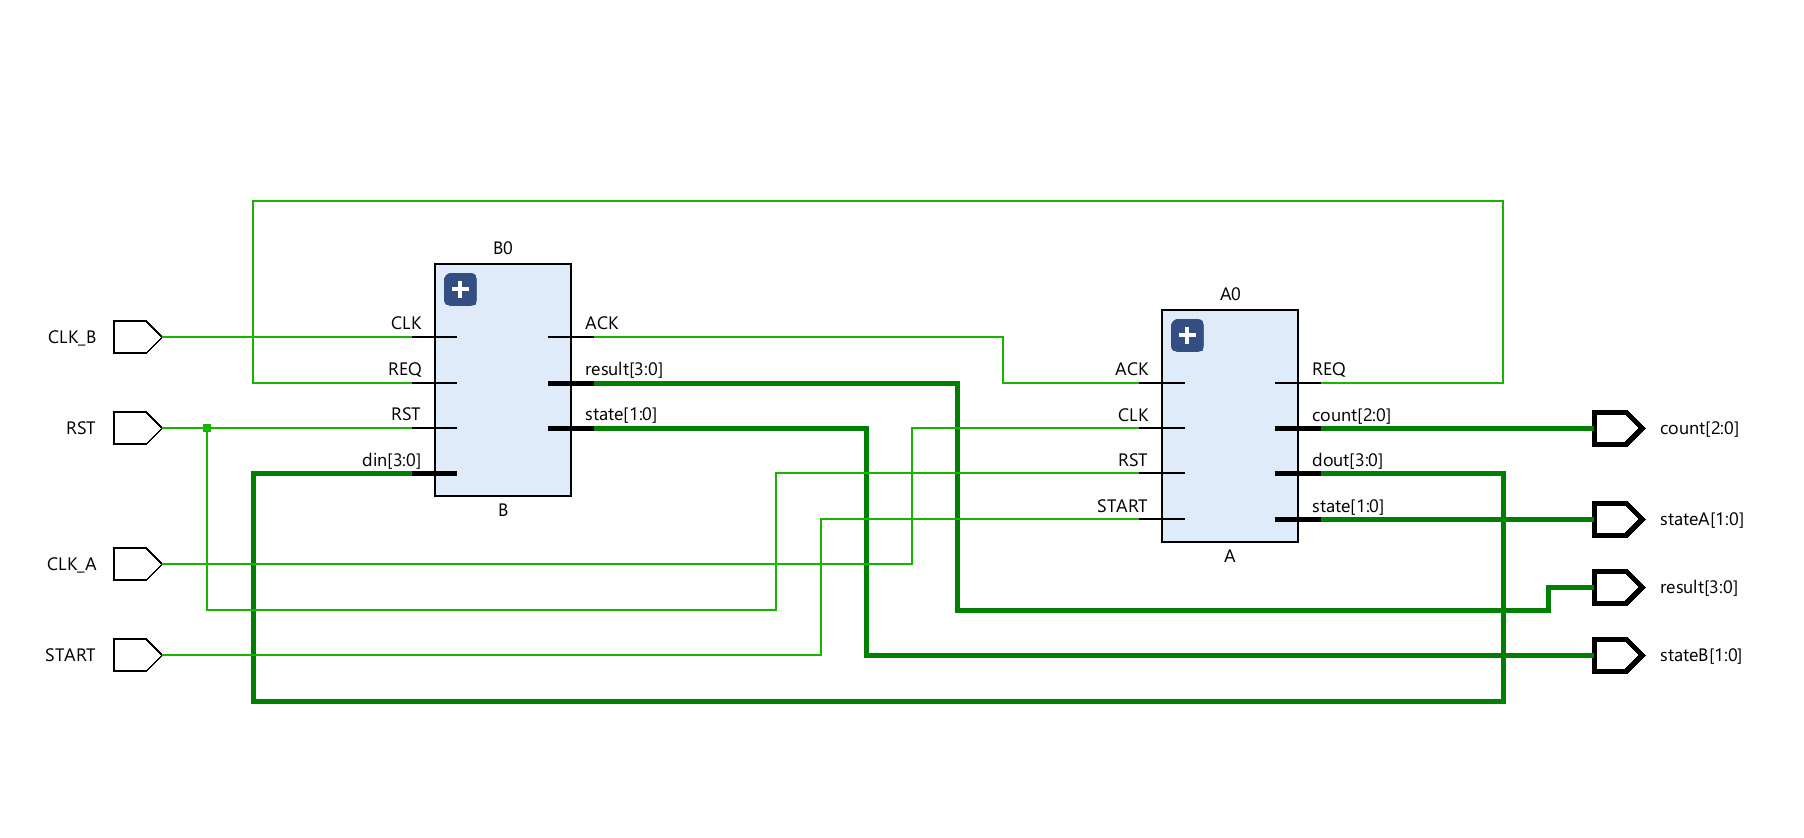
\includegraphics[width=1\textwidth]{img/preappDicembre/schematic_preapp}
	\caption{Schema a blocchi: nodo B}
	\label{wf_preapp} 
\end{figure}
\subsection{Simulazione}
Per procedere alla simulazione, è necessaria un testbench:
\begin{code}
    \inputminted[frame=lines, framesep=2mm, baselinestretch=1.2, bgcolor=LightGray, fontsize=\footnotesize, linenos]{vhdl}{vhdl_files/preappDicembre/testbench.vhd}
    \caption{testbench.vhdl}
    \label{lst:mux_2_1}
\end{code}
E eseguendo tale simulazione si ottiene la seguente waveform:
\begin{figure}[H]
	\centering
	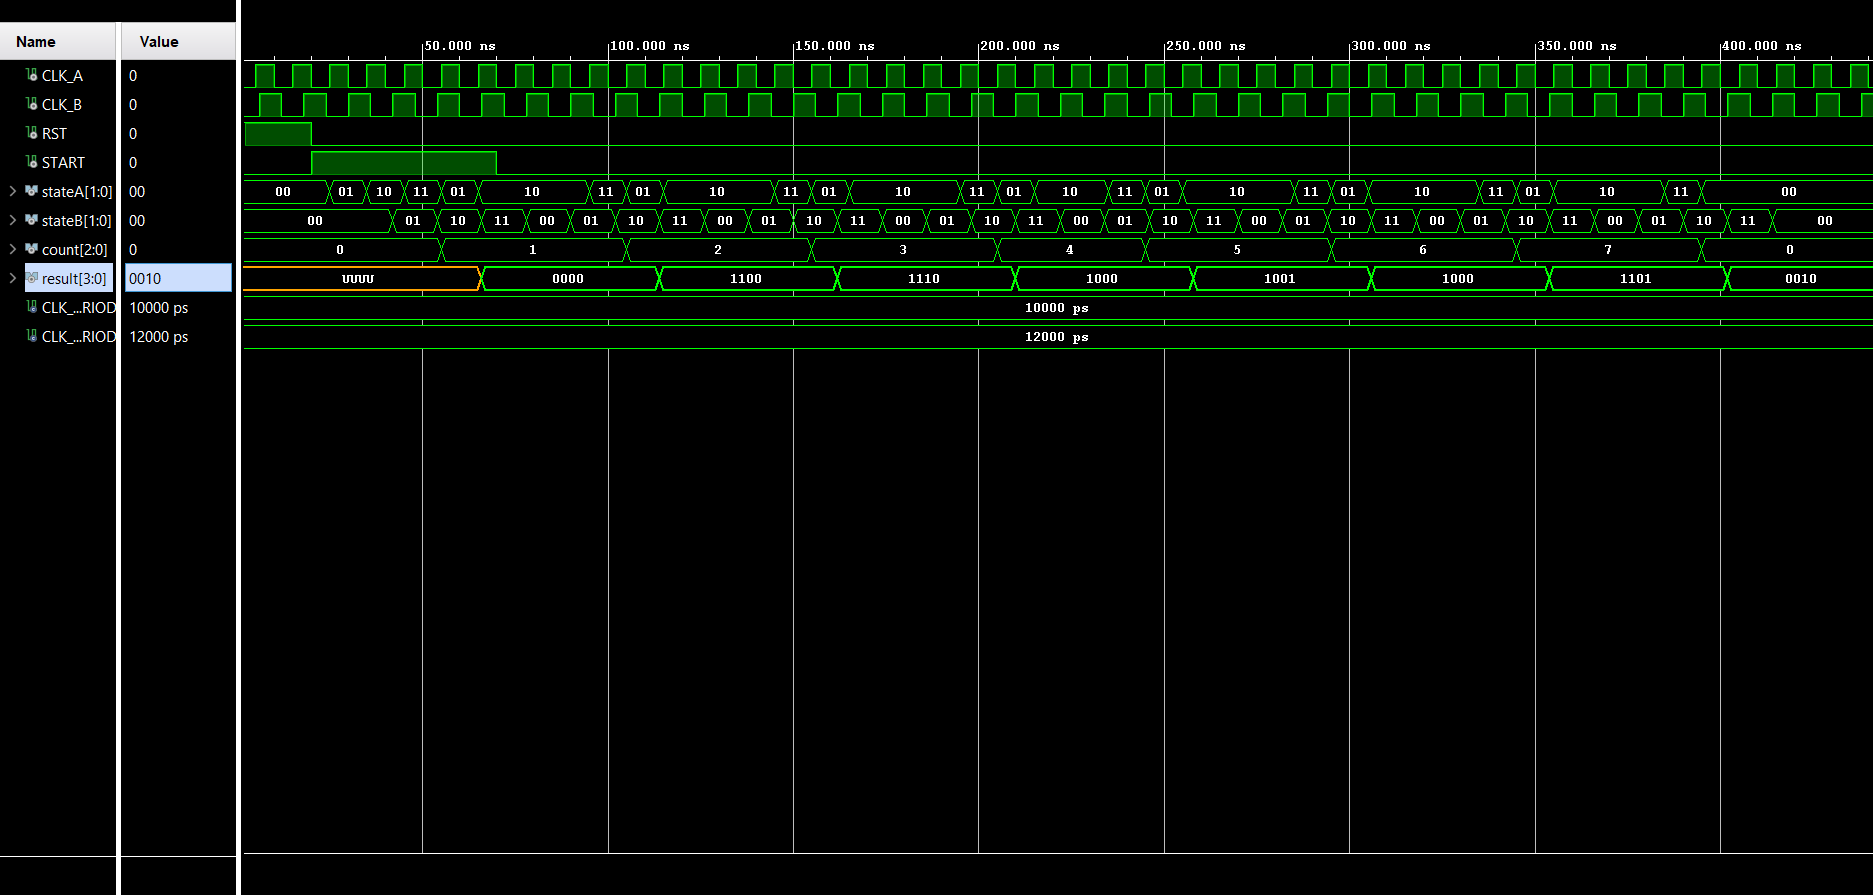
\includegraphics[width=1\textwidth]{img/preappDicembre/waveformPreappDic}
	\caption{Waveform}
	\label{wf_preapp} 
\end{figure}
Per valutare la correttezza della simulazione si ricordano gli elementi di ROM:
\begin{center}
\begin{tabbing}
0000 \=  \kill % Per definire l'allineamento
ROM[0] = 0000 \\
ROM[1] = 1100 \\
ROM[2] = 0010 \\
ROM[3] = 1010 \\
ROM[4] = 0001 \\
ROM[5] = 1111 \\
ROM[6] = 0101 \\
ROM[7] = 0011 \\
\end{tabbing}
\end{center}
Inizializzando il registro R a 0 e poi sommando progressivamente i valori a due a due si ottiene:
\begin{tabbing}
0000 \=  \kill % Per definire l'allineamento
0000 + 0000 = 0000\\
0000 + 1100 = 1100\\
1100 + 0010 = 1110\\
1110 + 1010 = 1000 \\
1000 + 0001 = 1001\\
1001 + 1111 = 1000 \\
1000 + 0101 = 1101 \\
\textbf{1101 + 0011 = 0010} \\
\end{tabbing}
Quindi alla fine sul registro sarà memorizzata la stringa 0010, che corrisponde alla somma di tutti gli elementi della ROM presente in A.